\documentclass{standalone}
\usepackage{tikz}
\usepackage{graphicx}
\usepackage{pgfmath}
\usetikzlibrary{backgrounds,shapes,arrows,positioning,calc,snakes,fit,arrows.meta}
\usepgflibrary{decorations.markings,decorations.text}
\tikzset{>=latex}

\begin{document}

\sffamily

  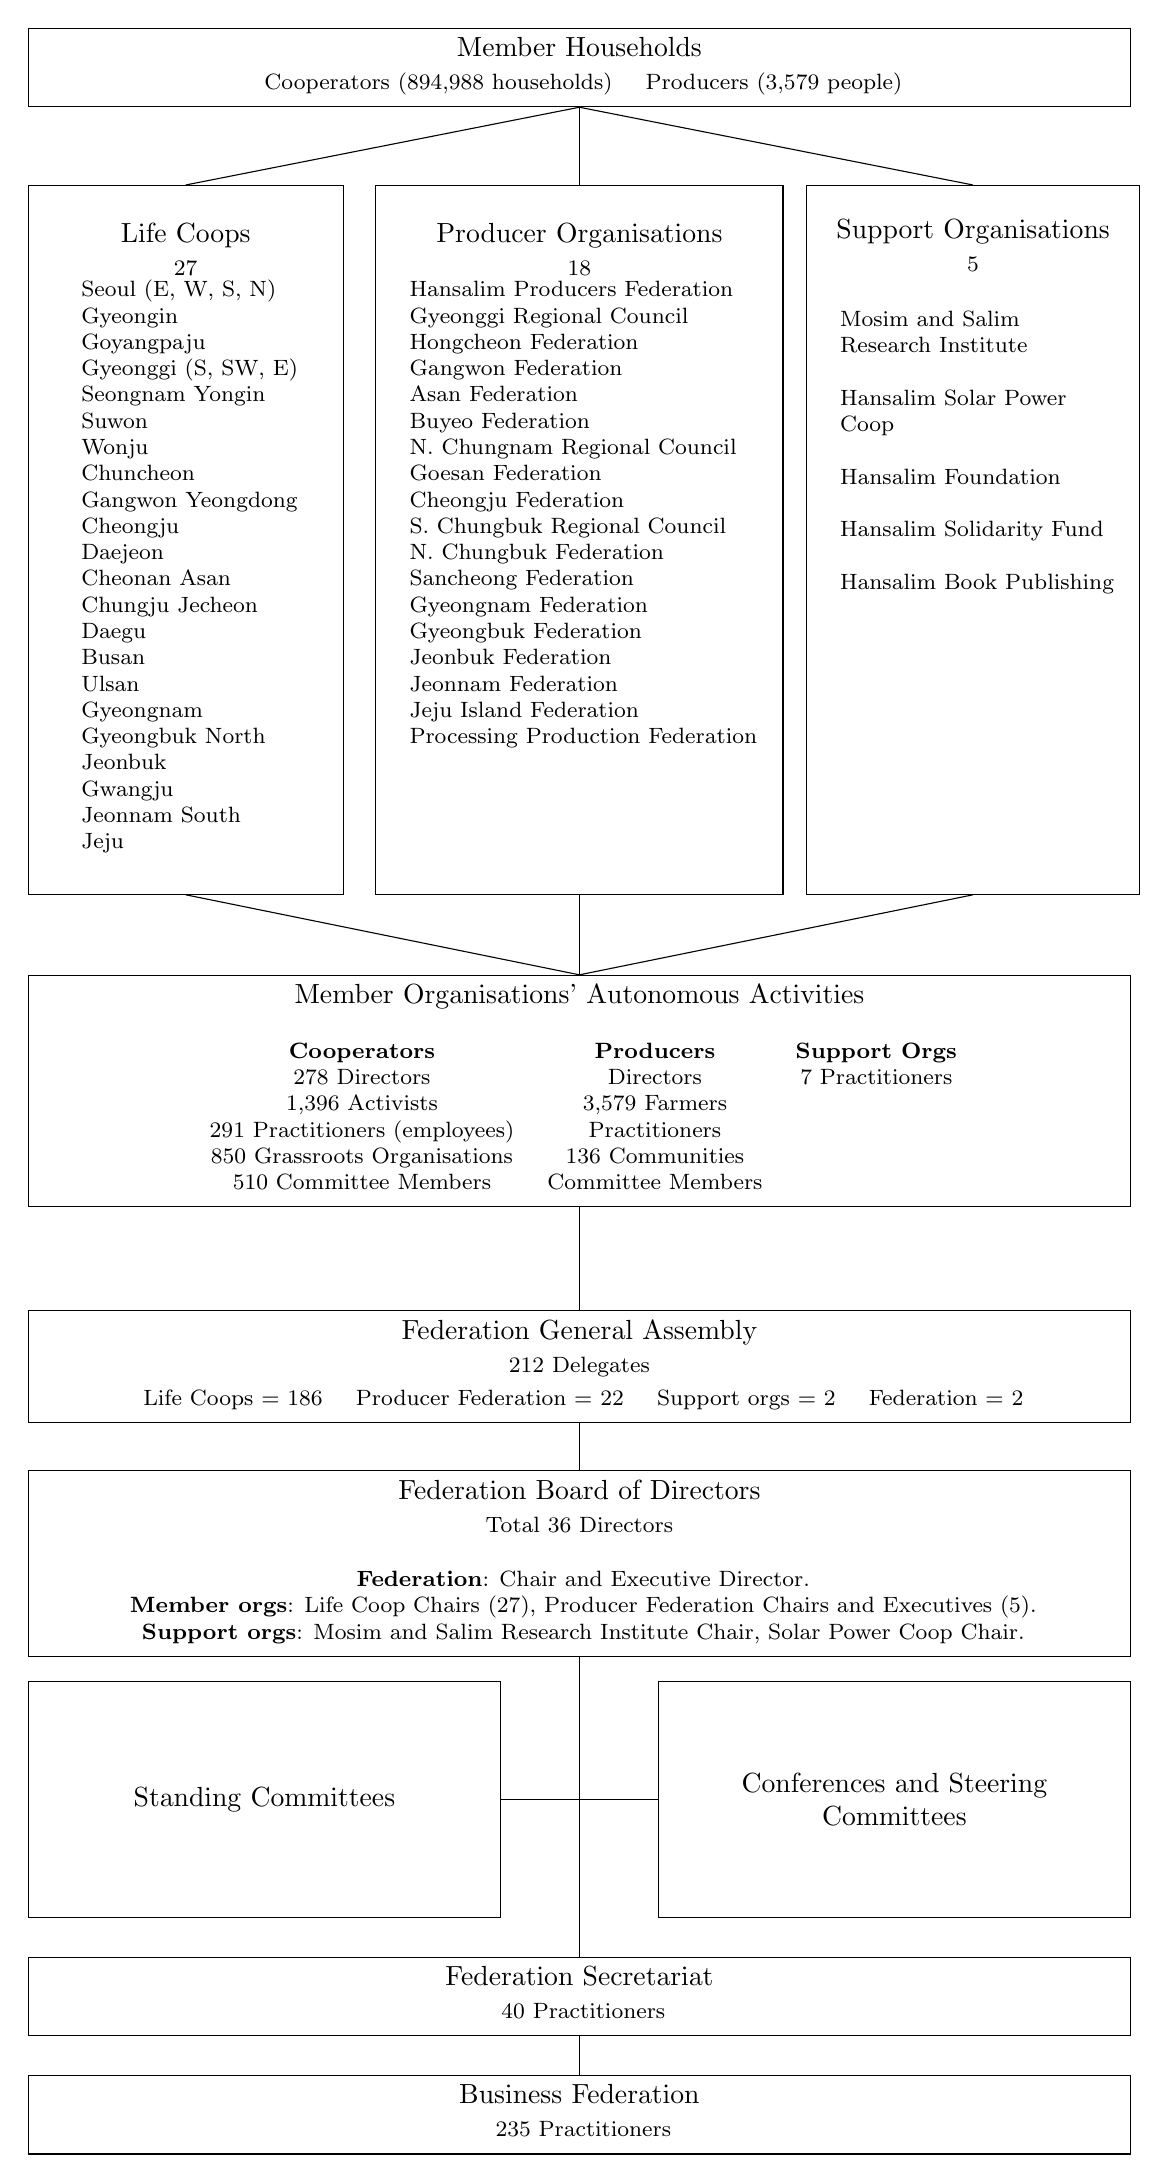
\begin{tikzpicture}

    \def\xLeft{2}
    \def\xCentre{7}
    \def\xRight{12}
    \def\xLeftMid{3}
    \def\xRightMid{11}
    \def\yOne{0}
    \def\yTwo{4}
    \def\yBusiness{1}
    \def\ySecretariat{2.5}
    \def\yCommittees{5}
    \def\yDirectors{8}
    \def\yAssembly{10.5}
    \def\yFederation{14}
    \def\yOrgs{21}
    \def\yHouseholds{27}

    \def\widthFull{14cm}
    \def\widthThird{4cm}
    \def\widthHalf{6cm}

    \def\heightBig{9cm}
    \def\heightMed{3cm}

    \node
        [minimum width=\widthFull,align=center,draw]
        at (\xCentre,\yHouseholds)
        (members) {Member Households\\
            \footnotesize{
            \begin{tabular}{cc}
                Cooperators (894,988 households) & Producers (3,579 people)\\ % Cooperators = 2024 GA p. 19 - 2023.12.31; Producers (including processing producers) = 2024 GA p. 24.
            \end{tabular}}};
    \node
        [minimum width=\widthThird,minimum height=\heightBig,align=center,draw]
        at (\xLeft,\yOrgs)
        (coops) {Life Coops\\\footnotesize{27}\\
            \footnotesize{
            \begin{tabular}{l}
                Seoul (E, W, S, N)\\ Gyeongin\\Goyangpaju\\Gyeonggi (S, SW, E)\\Seongnam Yongin\\Suwon\\Wonju\\Chuncheon\\Gangwon Yeongdong\\Cheongju\\Daejeon\\Cheonan Asan\\Chungju Jecheon\\Daegu\\Busan\\Ulsan\\Gyeongnam\\Gyeongbuk North\\Jeonbuk\\Gwangju\\Jeonnam South\\Jeju
            \end{tabular}}};
    \node
        [minimum width=\widthThird,minimum height=\heightBig,align=center,draw]
        at (\xCentre,\yOrgs)
        (producers) {Producer Organisations\\\footnotesize{18}\\
            \footnotesize{
            \begin{tabular}{l}
                Hansalim Producers Federation\\Gyeonggi Regional Council\\Hongcheon Federation\\Gangwon Federation\\Asan Federation\\Buyeo Federation\\N. Chungnam Regional Council\\Goesan Federation\\Cheongju Federation\\S. Chungbuk Regional Council\\N. Chungbuk Federation\\Sancheong Federation\\Gyeongnam Federation\\Gyeongbuk Federation\\Jeonbuk Federation\\Jeonnam Federation\\Jeju Island Federation\\Processing Production Federation\\ \\ \\ \\ \\
            \end{tabular}}};
    \node
        [minimum width=\widthThird,minimum height=\heightBig,align=center,draw]
        at (\xRight,\yOrgs)
        (support) {Support Organisations\\\footnotesize{5}\\\\
            \footnotesize{
            \begin{tabular}{l}
                Mosim and Salim\\Research Institute\\\\Hansalim Solar Power \\Coop\\\\Hansalim Foundation\\\\Hansalim Solidarity Fund\\\\Hansalim Book Publishing\\ \\ \\ \\ \\ \\ \\ \\ \\ \\ \\
            \end{tabular}}};
    \node
        [minimum width=\widthFull,align=center,draw]
        at (\xCentre,\yFederation)
        (federation) {Member Organisations' Autonomous Activities\\ \\
            \footnotesize{
            \begin{tabular}{ccc}
                \textbf{Cooperators} & \textbf{Producers} & \textbf{Support Orgs}\\
                278 Directors & Directors & 7 Practitioners \\ % from Miseong
                1,396 Activists & 3,579 Farmers & \\ %including Organisational activities, Store activities, Order consultation, Other (2024 GA p. 22-23).
                291 Practitioners (employees) & Practitioners & \\
                850 Grassroots Organisations & 136 Communities & \\ %including Neighbourhood gatherings, Small gatherings, Cooperator gatherings, Store gatherings, Branches, Local Steering Committees (2024 GA p. 22-23).
                510 Committee Members & Committee Members & %2024 GA p. 23 note 3.
            \end{tabular}}};
    \node
        [minimum width=\widthFull,align=center,draw]
        at (\xCentre,\yAssembly)
        (assembly) {Federation General Assembly\\\footnotesize{212 Delegates}\\
            \footnotesize{
                \begin{tabular}{cccc}
                Life Coops = 186 &
                Producer Federation = 22 &
                Support orgs = 2 &
                Federation = 2
                \end{tabular}}};
    \node
        [minimum width=\widthFull,align=center,draw]
        at (\xCentre,\yDirectors)
        (board) {Federation Board of Directors\\\footnotesize{Total 36 Directors}\\\\
            \footnotesize{
            \begin{tabular}{c}
            \textbf{Federation}: Chair and Executive Director. \\
            \textbf{Member orgs}: Life Coop Chairs (27), Producer Federation Chairs and Executives (5). \\
            \textbf{Support orgs}: Mosim and Salim Research Institute Chair, Solar Power Coop Chair.
            \end{tabular}}};
    \node
        [minimum width=\widthHalf,minimum height=\heightMed,align=center,draw]
        at (\xLeftMid,\yCommittees)
        (committees) {Standing Committees};
    \node
        [minimum width=\widthHalf,minimum height=\heightMed,align=center,draw]
        at (\xRightMid,\yCommittees)
        (conferences) {Conferences and Steering\\ Committees};
    \node
        [minimum width=\widthFull,align=center,draw]
        at (\xCentre,\ySecretariat)
        (secretariat) {Federation Secretariat\\
            \footnotesize{
            \begin{tabular}{c}
            40 Practitioners \\ % from Miseong
            \end{tabular}}};

    \node
        [minimum width=\widthFull,align=center,draw]
        at (\xCentre,\yBusiness)
        (business) {Business Federation\\
            \footnotesize{
            \begin{tabular}{c}
            235 Practitioners \\ % from Miseong
            \end{tabular}}};

    \draw[-] (members.south) -- (coops.north);
    \draw[-] (members.south) -- (producers.north);
    \draw[-] (members.south) -- (support.north);
    \draw[-] (coops.south) -- (federation.north);
    \draw[-] (producers.south) -- (federation.north);
    \draw[-] (support.south) -- (federation.north);
    \draw[-] (federation.south) -- (assembly.north);
    \draw[-] (assembly.south) -- (board.north);
    \draw[-] (board.south) -- (secretariat.north);
    \draw[-] (committees.east) -- (conferences.west);
    \draw[-] (secretariat.south) -- (business.north);

  \end{tikzpicture}

\end{document}
